\documentclass[a4paper]{article}
\usepackage{amsmath, amssymb, amsthm, mathrsfs, enumitem, tikz}
\usepackage[hmargin = 1in, vmargin = 1.25in]{geometry}
\title{Homework-12}
\author{Haocheng Wang \and 2019011994}

\newtheorem{ex}{Exercise}[subsection]
\newtheorem{lem}{Lemma}[subsection]
\stepcounter{section}
\setcounter{subsection}{6}
\renewcommand{\proofname}{\noindent\bf Proof}
\renewcommand\labelenumi{\roman}
\renewcommand{\Re}{\mathrm{Re}\,}
\renewcommand{\Im}{\mathrm{Im}\,}

\begin{document}
\maketitle
\setcounter{ex}{47}
\begin{ex}[Cantor function]\end{ex}\begin{proof}\ \begin{enumerate}[label = (\roman*)]
    \item Here is the graph of $F_0, F_1, F_2$.\begin{center}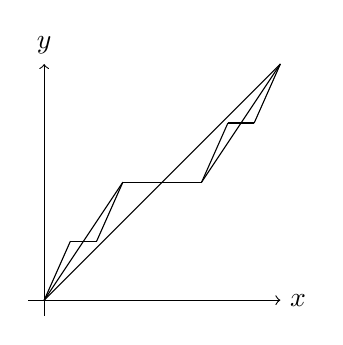
\begin{tikzpicture}
        \draw[->] (-0.2,0) --(3,0) node[right] {$x$};
        \draw[->] (0,-0.2) --(0,3) node[above] {$y$};
        \draw[domain=0:3] plot (\x ,{\x});
        \draw[domain=0:1] plot (\x, {1.5*\x});
        \draw[domain=1:2] plot (\x, {1.5});
        \draw[domain=2:3] plot (\x, {1.5*\x-1.5}); %F_1
        \draw[domain=0:1/3] plot (\x, {2.25*\x});
        \draw[domain=1/3:2/3] plot (\x, {3/4});
        \draw[domain=2/3:1] plot(\x, {2.25*\x-0.75});
        \draw[domain=2:7/3] plot(\x, {2.25*\x -3});
        \draw[domain=7/3:8/3] plot(\x, {9/4});
        \draw[domain=8/3:3] plot(\x, {2.25*\x-15/4});
    \end{tikzpicture}
\end{center}
    \item Note that $F_0$ is a continuous non-decreasing function with $F_0(0) = 0$ and $F_0(1) = 1$, now we induct
    on $n$, then from the definition of $F_{n + 1}$ we find that it's non-decreasing continuous, and 
    $F_{n + 1}(0) = \frac{1}{2}F_n(0) = 0, F_{n + 1}(1) = \frac{1}{2} + \frac{1}{2}F_n(3-2) = 1$.
    \item Note that for any $x \in [0, 1]$, one has that $|F_1(x) - F_0(x)| \leq 1$, then 
    by induction\begin{align*}
    &|F_{n + 1}(x) - F_n(x)| = |\frac{1}{2}F_n(3x) - \frac{1}{2}F_{n - 1}(3x)| \leq \frac{1}{2}2^{-(n - 1)} = 2^{-n}, \forall x \in [0, 1/3],\\
    &|F_{n + 1}(x) - F_n(x)| = |\frac{1}{2} + \frac{1}{2}F_n(3x - 2) - (\frac{1}{2} + \frac{1}{2}F_{n - 1}(3x - 2))|
    \leq  2^{-n}, \forall x \in [2/3, 1].
    \end{align*}
    Therefore $|F_{n + 1}(x) - F_n(x)| \leq 2^{-n}, \forall x \in [0, 1]$. Hence $F_n$ converge uniformly to a limit 
    $F : [0, 1] \to \mathbb{R}$.
    \item Let $\varepsilon > 0$, then there exists $N \in \mathbb{N}$ such that $|F_N(x) - F(x)| \leq \varepsilon/3$
    for any $x \in [0,1]$. Since $F_N$ is continuous, there exists $\delta > 0$ such that for any $|y - x| < \delta$
    one has $|F_N(y) - F_N(x)| \leq \varepsilon/3$. Given any $x \in [0,1]$, then for all $y$ with $|y - x| <\delta$
    one has $$
    |F(y) - F(x)| \leq |F(y) - F_N(y)| + |F_N(y) - F_N(x)| + |F_N(x) - F(x)| \leq 3\cdot\frac{\varepsilon}{3} = \varepsilon.
    $$Hence $F$ is continuous. Suppose for contradiction that there exists $y > x$ with $F(y) < F(x)$, i.e., 
    $F(x) - F(y) =: \lambda > 0$. So we can choose $N > 0$ such that $|F_N(x) - F(x)| < \lambda/3, \forall x \in [0,1]$,
    then$$
    F_N(y) - F_N(x) \leq (F(y) + \frac{\lambda}{3}) - (F(x) - \frac{\lambda}{3}) = -\frac{\lambda}{3} < 0.
    $$This contradiction implies that $F$ is monotone non-decreasing. Since $F_n(0) \equiv 0, F_n(1) \equiv 1$, we 
    have $F(0) = 0, F(1) = 1$.
    \item From the graph and definition of $F_n$ we find that $F_n$ is piecewisely constant outside $$
    I_n = \bigcup_{a_1,\dots, a_n \in \{0, 2\}}[\sum_{i = 1}^n \frac{a_i}{3^i}, \sum_{i = 1}^n \frac{a_i}{3^i} + \frac{1}{3^n}].
    $$And this implies $F_n$ is piecewisely constant outside $C = \bigcap_{n = 1}^\infty I_n$ known Cantor set. More
    precisely, if we define $$
    J_1 = (\frac{1}{3}, \frac{2}{3}),\ \ \ J_n = \frac{1}{3}J_{n - 1} \cup (\frac{1}{3} + J_{n - 1}),
    $$then for each $n$ one has $J_n = [0,1]\setminus I_n$ is the union of $2^n - 1$ open intervals, denote $J_n^{(k)}$ be the $k$th 
    component of $J_n$. Then we find that $F_n(x) = \frac{k}{2^n}, \forall x \in J_n^{(k)}$. Note that $J_n^{(k)} = J_{n + 1}^{(2k)}$,
    $F_n(x) = F_{n - 1}(x), \forall x \in J_{n - 1}$. Hence $F$ is piecewisely constant on $J = \bigcup_{n = 1}^\infty J_n$,
    which implies that if $x \in [0,1]$ lies outside $C$ one will find that $x \in J$ and thus $F$ is constant 
    in a neighbourhood of $x$, and in particular $F'(x) = 0$. Since $m(C) = 0$, one has $F'(x) = 0$ holds almost 
    everywhere, we conclude that $$
    \int_{[0,1]} F'(x)\,dx = 0\ne 1 = F(1) - F(0).
    $$
    \item This claim follows from the construction of $J_n$ in above.
    \item By construction we find that $|F(I)| = F_k(\sum_{i = 1}^n \frac{a_i}{3^i} + \frac{1}{3^n}) - F_k(\sum_{i = 1}^n \frac{a_i}{3^i})$
    whenever $k \geq n$. Note that $F_n$ is self-similar $|F(I)| = F(3^{-n}) - F(0) = 2^{-n}$.
    \item First we consider the right endpoints of $J_n$, e.g., we consider 
    $x = \sum_{i = 1}^{n - 1} a_i3^{-i} + 2\cdot 3^{-n}$. Now we let $3^{-(m + 1)} \leq h \leq  3^{-m}$, where $m > n$,
    thus $h \to 0$ as $m \to +\infty$. Therefore $$
    \frac{F(x + h) - F(x)}{h} \geq \frac{F(x + 3^{-(m + 1)}) - F(x)}{3^{-m}} = \frac{3^m}{2^{m + 1}} \to +\infty,
    $$which implies that $\overline{D^+}F(x) = +\infty$. Similarly one can show that any left endpoints of $J_n$ 
    is not differentiable. Hence $F$ is not differentiable at any element of the Cantor set $C$. \qedhere
\end{enumerate}
\end{proof}

\begin{ex}\end{ex}\begin{proof}\ \begin{enumerate}[label = (\roman*)]
    \item This is trivial.
    \item First we show that this is true for any sufficiently small interval. Suppose $F$ is absolutely continuous,
    then there exists $\delta > 0$ such that $\sum_{i = 1}^n |F(d_i) - F(c_i)| \leq 1$ whenever $(c_i, d_i)$ is a 
    finite collection of disjoint intervals lies in $[a, b]$ of total length $\sum_{i = 1}^n d_i - c_i \leq \delta$.
    Let $N = \lfloor \frac{b - a}{\delta}\rfloor + 1$, then divide $[a, b]$ into $N$ equal parts $[a_j, b_j]$.
    For each $j$, we have $\|F\|_{TV[a_j, b_j]}\leq 1$, finally by triangle inequality we obtain that 
    $\|F\|_{TV[a, b]} \leq N < \infty$.
    \item Suppose $C$ is the Lipschitz constant of function $F$, then for every $\varepsilon > 0$ we choose 
    $\delta < \varepsilon / C$. For any collection of disjoint intervals $(a_i, b_i)$ of total length less than $\delta$,
    one has $$
    \sum_{i = 1}^n |F(b_i) - F(a_i)| \leq \sum_{i = 1}^n C(b_i - a_i) \leq C\delta < \varepsilon.
    $$Hence Lipschitz continuous function is absolutely continuous.
    \item Given arbitary $\varepsilon > 0$, then set $\lambda = \varepsilon^2/4$. For any disjoint intervals $[a_i, b_i]$
    of total length $\sum_{i = 1}^n b_i - a_i \leq \varepsilon^2$, we break the sum $\sum_{i = 1}^n |\sqrt{b_i} - \sqrt{a_i}|$
    in two parts: those intervals that are in $[0, \lambda]$ and those in $[a, +\infty)$. If $\lambda$ happens to fall in the 
    middle of an interval we break the interval at $\lambda$, by triangle inequality this will only make the sum larger,
    and we denote $a_m = \lambda = b_m$. Then \begin{align*}
    &\sum_{i = 1}^m |\sqrt{b_i} - \sqrt{a_i}| \leq \sqrt{\lambda} \leq \frac{\lambda}{2},\\
    &\sum_{i = m + 1}^n |\sqrt{b_i} - \sqrt{a_i}| = \sum_{i = m + 1}^n |\sqrt{b_i} - \sqrt{a_i}|\cdot 
    \frac{|\sqrt{b_i} + \sqrt{a_i}|}{|\sqrt{b_i} + \sqrt{a_i}|} = \sum_{i = m + 1}^n\frac{b_i - a_i}{|\sqrt{b_i} + \sqrt{a_i}|}\\
    &\leq \sum_{i = m + 1}^n \frac{b_i - a_i}{2\sqrt{\lambda}} = \frac{1}{\varepsilon}\cdot \varepsilon^2 = \varepsilon.
    \end{align*}
    Hence $\sum_{i = 1}^n |\sqrt{b_i} - \sqrt{a_i}| \leq 2\varepsilon$, which implies that $x \mapsto \sqrt{x}$ is absolutely
    continuous. However, this function cannot be Lipschitz continuous, for its derivative $\frac{1}{2\sqrt{x}}$ 
    is not bounded.
    \item Since any continuous function on a compact interval is uniformly continuous, so is Cantor function.
    To show that Cantor function $F$ is not absolutely continuous, we consider $I_n$ which is consists of $2^n$
    intervals, and we denote their endpoints in turn, we have $F(b_i) = F(a_{i + 1})$ and thus$$
    \sum_{i = 1}^{2^n} |F(b_i) - F(a_i)| = \sum_{i = 1}^{2^n} F(b_i) - F(a_i) = F(1) - F(0) \equiv 1.
    $$However $|I_n| = (\frac{2}{3})^n \to 0$ as $n \to \infty$, hence $F$ is not absolutely continuous.
    \item For arbitary $\varepsilon > 0$, since $f$ is absolutely integrable, by dominated convergence theorem 
    $$
    \lim_{M \to \infty} \int_{\mathbb{R}}f(x)1_{|f| \geq M}(x)\,dx = 
    \int_{\mathbb{R}}f(x)\lim_{M \to \infty} 1_{|f| \geq M}(x)\,dx = 0.
    $$Therefore we can choose $M > 0$ such that $\int_{\mathbb{R}}|f(x)1_{|f| \geq M}(x)|\,dx \leq \varepsilon / 2$.
    Then for any collection of disjoint intervals $[a_i, b_i] \subset \mathbb{R}$ of total length 
    $\sum_{i = 1}^n b_i - a_i \leq \varepsilon / 2M$, one has \begin{align*}
    \sum_{i = 1}^n |F(b_i) - F(a_i)| &\leq \sum_{i = 1}^n \int_{[a_i, b_i]} |f(x)(1_{|f| < M}(x) + 1_{|f| \geq M}(x))|\,dx\\
    &\leq \sum_{i = 1}^n M(b_i - a_i) + \int_{\mathbb{R}} |f(x)1_{|f| \geq M}(x)|\,dx \leq \varepsilon.
    \end{align*}
    Hence $F(x)$ is absolutely continuous. By (ii), $F$ is differentiable almost everywhere; since $f$ is absolutely
    integrable, $F'(x) = f(x)$ for almost everywhere $x$.
    \item Let $f$ and $g$ be two absolutely continuous function, first we show that $f + g$ is absolutely continuous.
    By definition, for every $\varepsilon > 0$, there exists $\delta_f, \delta_g > 0$ such that for any collection of
    disjoint intervals $[a_i, b_i]$ satisfying total length less than $\delta_f$ one has $\sum_{i = 1}^n |f(b_i) - f(a_i)| < \varepsilon/2$,
    and similar for $g$. Now we set $\delta = \min(\delta_f, \delta_g)$, then for any collection whose length less than
    $\delta$ one has $$
    \sum_{i = 1}^n |f(b_i) + g(b_i) - f(a_i) - g(a_i)| \leq \sum_{i = 1}^n |f(b_i) - f(a_i)| + \sum_{i = 1}^n 
    |g(b_i) - g(a_i)| \leq \varepsilon.
    $$Hence $f + g$ is absolutely continuous. To show that $fg$ is also absolutely continuous on $[a, b]$, note that
    there exists $M_f, M_g > 0$ such that $|f(x)|\leq M_f, |g(x)| \leq M_g, \forall x \in [a, b]$, we turn to choose
    $\delta_f$ and $\delta_g$ respectively such that $\sum_{i = 1}^n |f(b_i) - f(a_i)| \leq \varepsilon/2M_g$
    and $\sum_{i = 1}^n |g(b_i) - g(a_i)| \leq \varepsilon/2M_f$. Now for any collection of total length less than 
    $\delta = \min(\delta_f, \delta_g)$ we have \begin{align*}
    \sum_{i = 1}^n |f(b_i)g(b_i) - f(a_i)g(a_i)| &\leq \sum_{i = 1}^n |g(b_i)||f(b_i) - f(a_i)| + \sum_{i = 1}^n
    |f(a_i)||g(b_i) - g(a_i)|\\
    &\leq M_g\sum_{i = 1}^n |f(b_i) - f(a_i)| + M_f\sum_{i = 1}^n |g(b_i) - g(a_i)| \leq \varepsilon.
    \end{align*}
    Hence $fg$ is also absolutely continuous.
\end{enumerate}
\end{proof}

\stepcounter{ex}\begin{ex}\end{ex}\begin{proof}
By Exercise 1.6.49 we know that $\int_{[a, x]}f(y)\,dy + C$ where $f$ is absolutely integrable function is absolutely
continuous, it suffices to show the reverse. Given an absolutely continuous function $F$, then $F$ is differentiable
almost everywhere and $F'$ is absolutely integrable, then by Second fundamental theorem we have $\int_{[a, x]}F'(x)\,dx = F(x) - F(a)$,
which implies that $F(x) = \int_{[a,x]}F'(x)\,dx + F(a)$.
\end{proof}

\stepcounter{ex}\begin{ex}\end{ex}\begin{proof}
Directly compute: $\lim_{h \to 0} \frac{F(h) - F(0)}{h} = \lim_{h\to 0}h\sin(\frac{1}{h^3}) = 0$. Hence $F$ is 
everywhere differentiable, its derivative$$
F'(x) = \begin{cases}
    0, &\text{if}\ \ x = 0,\\
    -\frac{3}{x^2}\cos(\frac{1}{x^3}) + 2x\sin(\frac{1}{x^3}), &\text{if}\ \ x \in [-1, 1]\setminus\{0\}.
\end{cases}
$$
Since $|2x\sin(\frac{1}{x^3})| \leq |2x|$ which is absolutely integrable, it suffices to verify that 
$\frac{3}{x^2}\cos(\frac{1}{x^3})$ is not absolutely integrable on $[-1,1]$. For large $k$, one has 
$I_k := [(2k\pi + \frac{\pi}{4})^{-1/3}, (2k\pi - \frac{\pi}{4})^{-1/3}] \subset [-1,1]$, and \begin{align*}
\int_{I_k} |\frac{3}{x^2}\cos(\frac{1}{x^3})|\,dx &\geq \frac{3}{\sqrt{2}}(2k\pi- \frac{\pi}{4})^{2/3}
((2k\pi - \frac{\pi}{4})^{-1/3} - (2k\pi + \frac{\pi}{4})^{-1/3})\\
&= \frac{3}{\sqrt{2}}(2k\pi - \frac{\pi}{4})^{1/3}\Bigg(1 - \sqrt[3]{1 - \frac{2}{8k + 1}}\Bigg)
\geq \frac{3}{\sqrt{2}}(2k\pi - \frac{\pi}{4})^{1/3}\Bigg(1 - (1 - \frac{1}{3}\cdot\frac{2}{8k + 1})\Bigg)\\
&= \sqrt{2}(\frac{\pi}{4})^{1/3}\frac{\sqrt[3]{8k-1}}{8k + 1} \sim \frac{1}{k^{2/3}}.
\end{align*}
Therefore $$
\int_{[-1,1]}|F'(x)|\,dx \geq \sum_{k = 1}^\infty \sqrt{2}(\frac{\pi}{4})^{1/3}\frac{\sqrt[3]{8k-1}}{8k + 1} = +\infty.
$$Hence $F'$ is not absolutely integrable.
\end{proof}

\begin{ex}[Henstock-Kurzweil integral]\end{ex}\begin{proof}\ \begin{enumerate}[label = (\roman*)]
    \item Suppose $f$ is Henstock-Kurzweil integrable with integral $L_1$ and $L_2$. Then for any $\varepsilon > 0$,
    by definition there exists two gauge function $\delta_1$ and $\delta_2$, so we set $\delta = \min(\delta_1, \delta_2)$
    which is another gauge function. By Cousin's theorem there exists a partition $a = t_0 < t_1 < \cdots < t_k = b$
    equipped with distinguished point $t_1^*, \dots, t_k^*$ that $t_j^* \in [t_{j - 1}, t_j]$ and 
    $|t_j - t_{j - 1}| \leq \delta(t_j^*) \leq \delta_i(t_j^*), i = 1,2$. Therefore  $$
    |L_1 - L_2| \leq |\sum_{j = 1}^k f(t_j^*)(t_j - t_{j - 1}) - L_1| + |\sum_{j = 1}^k f(t_j^*)(t_j - t_{j - 1}) - L_2|
    \leq 2\varepsilon.
    $$Since $\varepsilon$ is arbitary, we obtain that $L_1 = L_2$.
    \item Since $f$ is Riemann integrable, for every $\varepsilon > 0$ there exists $\delta > 0$ such that 
    $|\mathcal{R}(f; \mathcal{P}) - \int_a^b f(x)\,dx| \leq \varepsilon$ whenever the the \emph{mesh} $\Delta(\mathcal{P})$ of partition 
    $\mathcal{P}$ is no more than $\delta$. Hence if we set the gauge function $\delta(x) \equiv \delta$, we find 
    that $f$ is Henstock-Kurzweil integrable, and by uniqueness we obtain that $\int_{[a, b]}f(x)\,dx = \int_a^b f(x)\,dx$.
    \item Define $F(x) = \int_{[a,x]}f(t)\,dt$ and thus $F$ is absolutely continuous and almost everywhere differentiable.
    Now let $\varepsilon > 0$, then we can find a $\kappa > 0$ small enough such that $\sum_{j = 1}^n |F(b_j) - F(a_j)| \leq \varepsilon$
    whenever $(a_1, b_1), \dots, (a_n, b_n)$ is a finite collection of disjoint intervals of total length 
    $\sum_{j = 1}^n b_j - a_j$ at most $\kappa$. Let $E \subset [a, b]$ be the set of point $x$ where $x$ is not a Lebesgue point of $f$, 
    together with the endpoints $a, b$; thus $E$ is a null set. 

    For every natural number $m = 1,2,\dots$ we can find an open set $U_m$ containing $E$ of measure $m(U_m) < \kappa/4^m$.
    In particular, we see that $m(\bigcup_{m = 1}^\infty U_m) \leq \kappa$.
    
    Now we define a gauge function $\delta: [a, b] \to (0, +\infty)$ as follows:\begin{enumerate}[label = (\alph*)]
        \item If $x \in E$, we define $\delta(x) > 0$ to be a small enough number such that the open interval 
        $(x - \delta(x), x + \delta(x))$ lies in $U_m$, where $m$ is the first natural number such that $|f(x)| \leq 2^m$.
        \item If $x \not\in E$, we let $\delta(x) > 0$ be small enough number such that $|F(y) - F(x) - (y - x)f(x)| \leq \varepsilon |y - x|$
        holds whenever $|y - x| \leq \delta(x)$.
    \end{enumerate}
    Applying Cousin's theorem, we can find a partition $a = t_0 < t_1 < \cdots < t_k =  b$ with $k \geq 1$, together
    with real number $t_j^* \in [t_{j - 1}, t_j]$ for each $1 \leq j \leq k$ and $t_j - t_{j - 1} \leq \delta(t_j^*)$.
    By construction, we have $$
    \sum_{j: t_j^* \in E} |F(t_j) - F(t_{j - 1})| \leq \varepsilon
    $$and thus $$
    \sum_{j: t_j^* \in E} F(t_j) - F(t_{j - 1}) = O(\varepsilon).
    $$Next we consider those $j$ for which $t_j^* \not\in E$. By construction, for those $j$ we have $$
    F(t_j) - F(t_{j - 1}) = f(t_j^*)(t_j - t_{j - 1}) + O(\varepsilon |t_j - t_{j - 1}|)
    $$and thus $$
    \sum_{j: t_j^* \not\in E} F(t_j) - F(t_{j - 1}) = \sum_{j: t_j^* \not\in E} f(t_j^*)(t_j - t_{j - 1}) + O(\varepsilon|b - a|).
    $$On the other hand$$
    \sum_{j: t_j^* \in E} f(t_j^*)(t_j - t_{j - 1}) \leq \sum_{m = 1}^\infty 2^m m(U_m) \leq \sum_{m = 1}^\infty
    2^m\varepsilon/4^m = O(\varepsilon).
    $$Putting everything together, we conclude that$$
    \int_{[a, b]} f(x)\,dx = F(b) = \sum_{j = 1}^k F(t_j) - F(t_{j - 1}) = \sum_{j = 1}^k f(t_j^*)(t_j - t_{j - 1})
    + O(\varepsilon) + O(\varepsilon |b - a|).
    $$Hence $f$ is Henstock-Kurzweil integrable, and the Henstock-Kurzweil integral is equal to the
    Lebesgue integral $\int_{[a, b]} f(x)\,dx$.
    \item We use the definition of gauge function in Proposition 1.6.41., by the similar argument in (iii) and the claim follows.
    \item Given $F'(x) = G'(x)$, then \[
        F(x) = \int_{[a,x]} F'(x)\,dx + F(a) = \int_{[a,x]} G'(x)\,dx + G(a) + F(a) - G(a) = G(x) + F(a) - G(a).
        \]This proves Theorem 1.6.40. Given everywhere differentiable function $F$, then $F'$ is Riemann integrable, 
        further by compatibility with the Riemann integral of Lebesgue integral we obtain 
        $\int_{[a,b]}F'(x)\,dx\ (\mathrm{L}) = \int_a^b F'(x)\,dx = \int_{[a,b]} F'(x)\,dx\ (\mathrm{H}\text{-}\mathrm{K}) = F(b) - F(a)$.
        \qedhere
\end{enumerate}
\end{proof}

(6)\begin{proof}
\ \begin{enumerate}[label = (\alph*)]
    \item By vertical truncation we may assume that $E$ is compact. Since $f = f^+ - f^-$ we may assume that $f$ is 
    non-negative; note that $f$ is measurable, there exists a sequence of unsigned simple functions $\{g_n\}_{n \geq 1}$
    such that $g_n \uparrow f$. Since $|f - g_n|^p \leq |f|^p$, we apply dominated convergence theorem and obtain$$
    \lim_{n \to \infty} \|f - g_n\|_{L^p(E)} = \lim_{n \to \infty} \int_E |f(x) - g_n(x)|^p\,dx = 
    \int_E \lim_{n\to\infty} |f(x) - g_n(x)|^p\,dx = 0.
    $$Hence for every $\varepsilon > 0$ there exists a compact supported function $g(x)$ such that 
    $\|f - g\|_{L^p(E)} \leq \varepsilon$.
    \item By triangle inequality we may assume that $f = 1_F$ where $F \subset E$ is measurable. But any Lebesgue
    measurable set $F$ is almost dyadically elementary and the claim follows.\qedhere
\end{enumerate}
\end{proof}
\end{document}